\documentclass{article}

\usepackage{preamb}

\usepackage[english]{babel}
\usepackage[utf8]{inputenc}
\usepackage[backend=biber,style=verbose,citetracker=true]{biblatex}
\usepackage[T1]{fontenc}
\usepackage{csquotes}

\graphicspath{{../images/}}
\addbibresource{bibliography.bib}

\author{Tanguy Lefort}
\title{Title}


%%%%%%%%%%%%%%%%%%%%%%%%%%%%%%%%%%%%%%%%%%%%%%%%%%%%%%%%%%%%%%%%%%%%
%%%%%%%%%%%%%%%%%%%% Begin document - title page %%%%%%%%%%%%%%%%%%%
%%%%%%%%%%%%%%%%%%%%%%%%%%%%%%%%%%%%%%%%%%%%%%%%%%%%%%%%%%%%%%%%%%%%


\begin{document}

\begin{titlepage} 
	\newcommand{\HRule}{\rule{\linewidth}{0.5mm}}
	
	\center
	
	\textsc{\LARGE University of Montpellier}\\[1.5cm]
	
	\textsc{\Large Master 2 Biostatistics }\\[0.5cm] 
	
	\textsc{\large HMMA$307$ project}\\[0.5cm] 
    \vspace{2cm}
	\HRule\\[0.4cm]
	
	{\huge\bfseries Sparse Regularization via Bidualization}\\[0.4cm] 
	
	\HRule\\[1.5cm]
	
	\begin{minipage}{0.4\textwidth}
		\begin{flushleft}
			\large
			\textit{By:}\\
			Tanguy Lefort 
		\end{flushleft}
	\end{minipage}
	~
	\begin{minipage}{0.4\textwidth}
		\begin{flushright}
			\large
			\textit{Teacher: }\\
			Joseph salmon\\
		\end{flushright}
	\end{minipage}
	\vspace{2cm}
	\vfill % Position the date 3/4 down the remaining page
	
	{\large 2020} 
	\begin{tikzpicture}[remember picture,overlay]
    \node[anchor=south] at (current page text area.south) {
\includegraphics[scale=0.3]{Logo.pdf}};
    \end{tikzpicture}	
	 
	%----------------------------------------------------------------------------------------
	
	\vfill 
\end{titlepage}

\tableofcontents

%%%%%%%%%%%%%%%%%%%%%%%%%%%%%%%%%%%%%%%%%%%%%%%%%%%%%%%%%%%%%%%%%%%%
% Introduction
%%%%%%%%%%%%%%%%%%%%%%%%%%%%%%%%%%%%%%%%%%%%%%%%%%%%%%%%%%%%%%%%%%%%

\section*{Introduction}

The increasing................


%%%%%%%%%%%%%%%%%%%%%%%%%%%%%%%%%%%%%%%%%%%%%%%%%%%%%%%%%%%%%%%%%%%%
% Sections of presentation
%%%%%%%%%%%%%%%%%%%%%%%%%%%%%%%%%%%%%%%%%%%%%%%%%%%%%%%%%%%%%%%%%%%%

\section{Solving problems with regularization}

% Present the problem with existing ridge and why L0
Regularized problems are a very useful way to obtain a solution in many situations. We write the problem as 
\[\min_{x\in\RR^n} f(x) + \mathrm{pen}(x)\enspace,\]
where $f$ only depends of the data collected and $\mathrm{pen}$ is a penalty term. It can represent for example a constraint over the number of variables that play a role.
In the case of the Tikhonov-ridge regularization, for a matrix $A\in\RR^{n\times n}$ made from the data and an observed signal $b\in\RR^n$, we write the problem
\[\min_{x\in\RR^n} \frac{1}{2}\|Ax-b\|^2_2 + \frac{\lambda}{2}\|x\|^2_2\enspace,\]
where $\lambda \geq 0$ represents how strong the penalty on the $l_2$ norm of the solution is. Note that for $\lambda = 0$ we retrieve the least square problem, and when $\lambda\rightarrow +\infty$, we have $x=0$.
However, when working with an observed signal, we sometimes know in advance the sparsity (or a reasonable estimate) of the original one. So we have an information that is stronger than a constraint on the norm of the vector, we have a constraint on the number of non-zero values, meaning on the $l_0$ norm.

% define the l_0 norm and space Ck
\begin{definition}
Let $x\in\RR^n$, the $l_0$ norm of $x$ noted $\|x\|_0$ is the number of non-zero values: \[\|x\|_0:=\abs{\{i\,|\, x_i\neq 0\}}\enspace .\]
We note $C_k$ the space of the $k$-sparse vectors: $C_k := \{x\in\RR^n\,|\, \|x\|_0 = k\}.$
\end{definition}

% introduce LASSO and ENET
One of the main advantages of the Tikhonov ($l_2$) regularization is the differentiability, the convexity and the continuity. With the $l_0$ norm, we lose them all. This lead to a compromise called the \lasso using the $l_1$ norm to keep the continuity and use sub-differentials instead of regular ones. The \lasso method will select some variables (depending on the value of $\lambda$) to explain the observed signal. It is very useful in a lot of situations like in genomics, but in situations with highly correlated groups of variables, the \lasso tends to only select one from each group and force the others to a null-effect as we can see on Figure \ref{fig:lasso_enet}. This issue lead to the development of the \enet method which uses a penalizer that is a combination of the Tikhonov and \lasso penalty
\[\min_{x\in\RR^n} \frac{1}{2}\|Ax-b\|^2_2 + \lambda_1 \|x_1\| +  \frac{\lambda_2}{2}\|x\|^2_2\enspace.\]

\begin{center}
    \begin{figure}
        \centering
        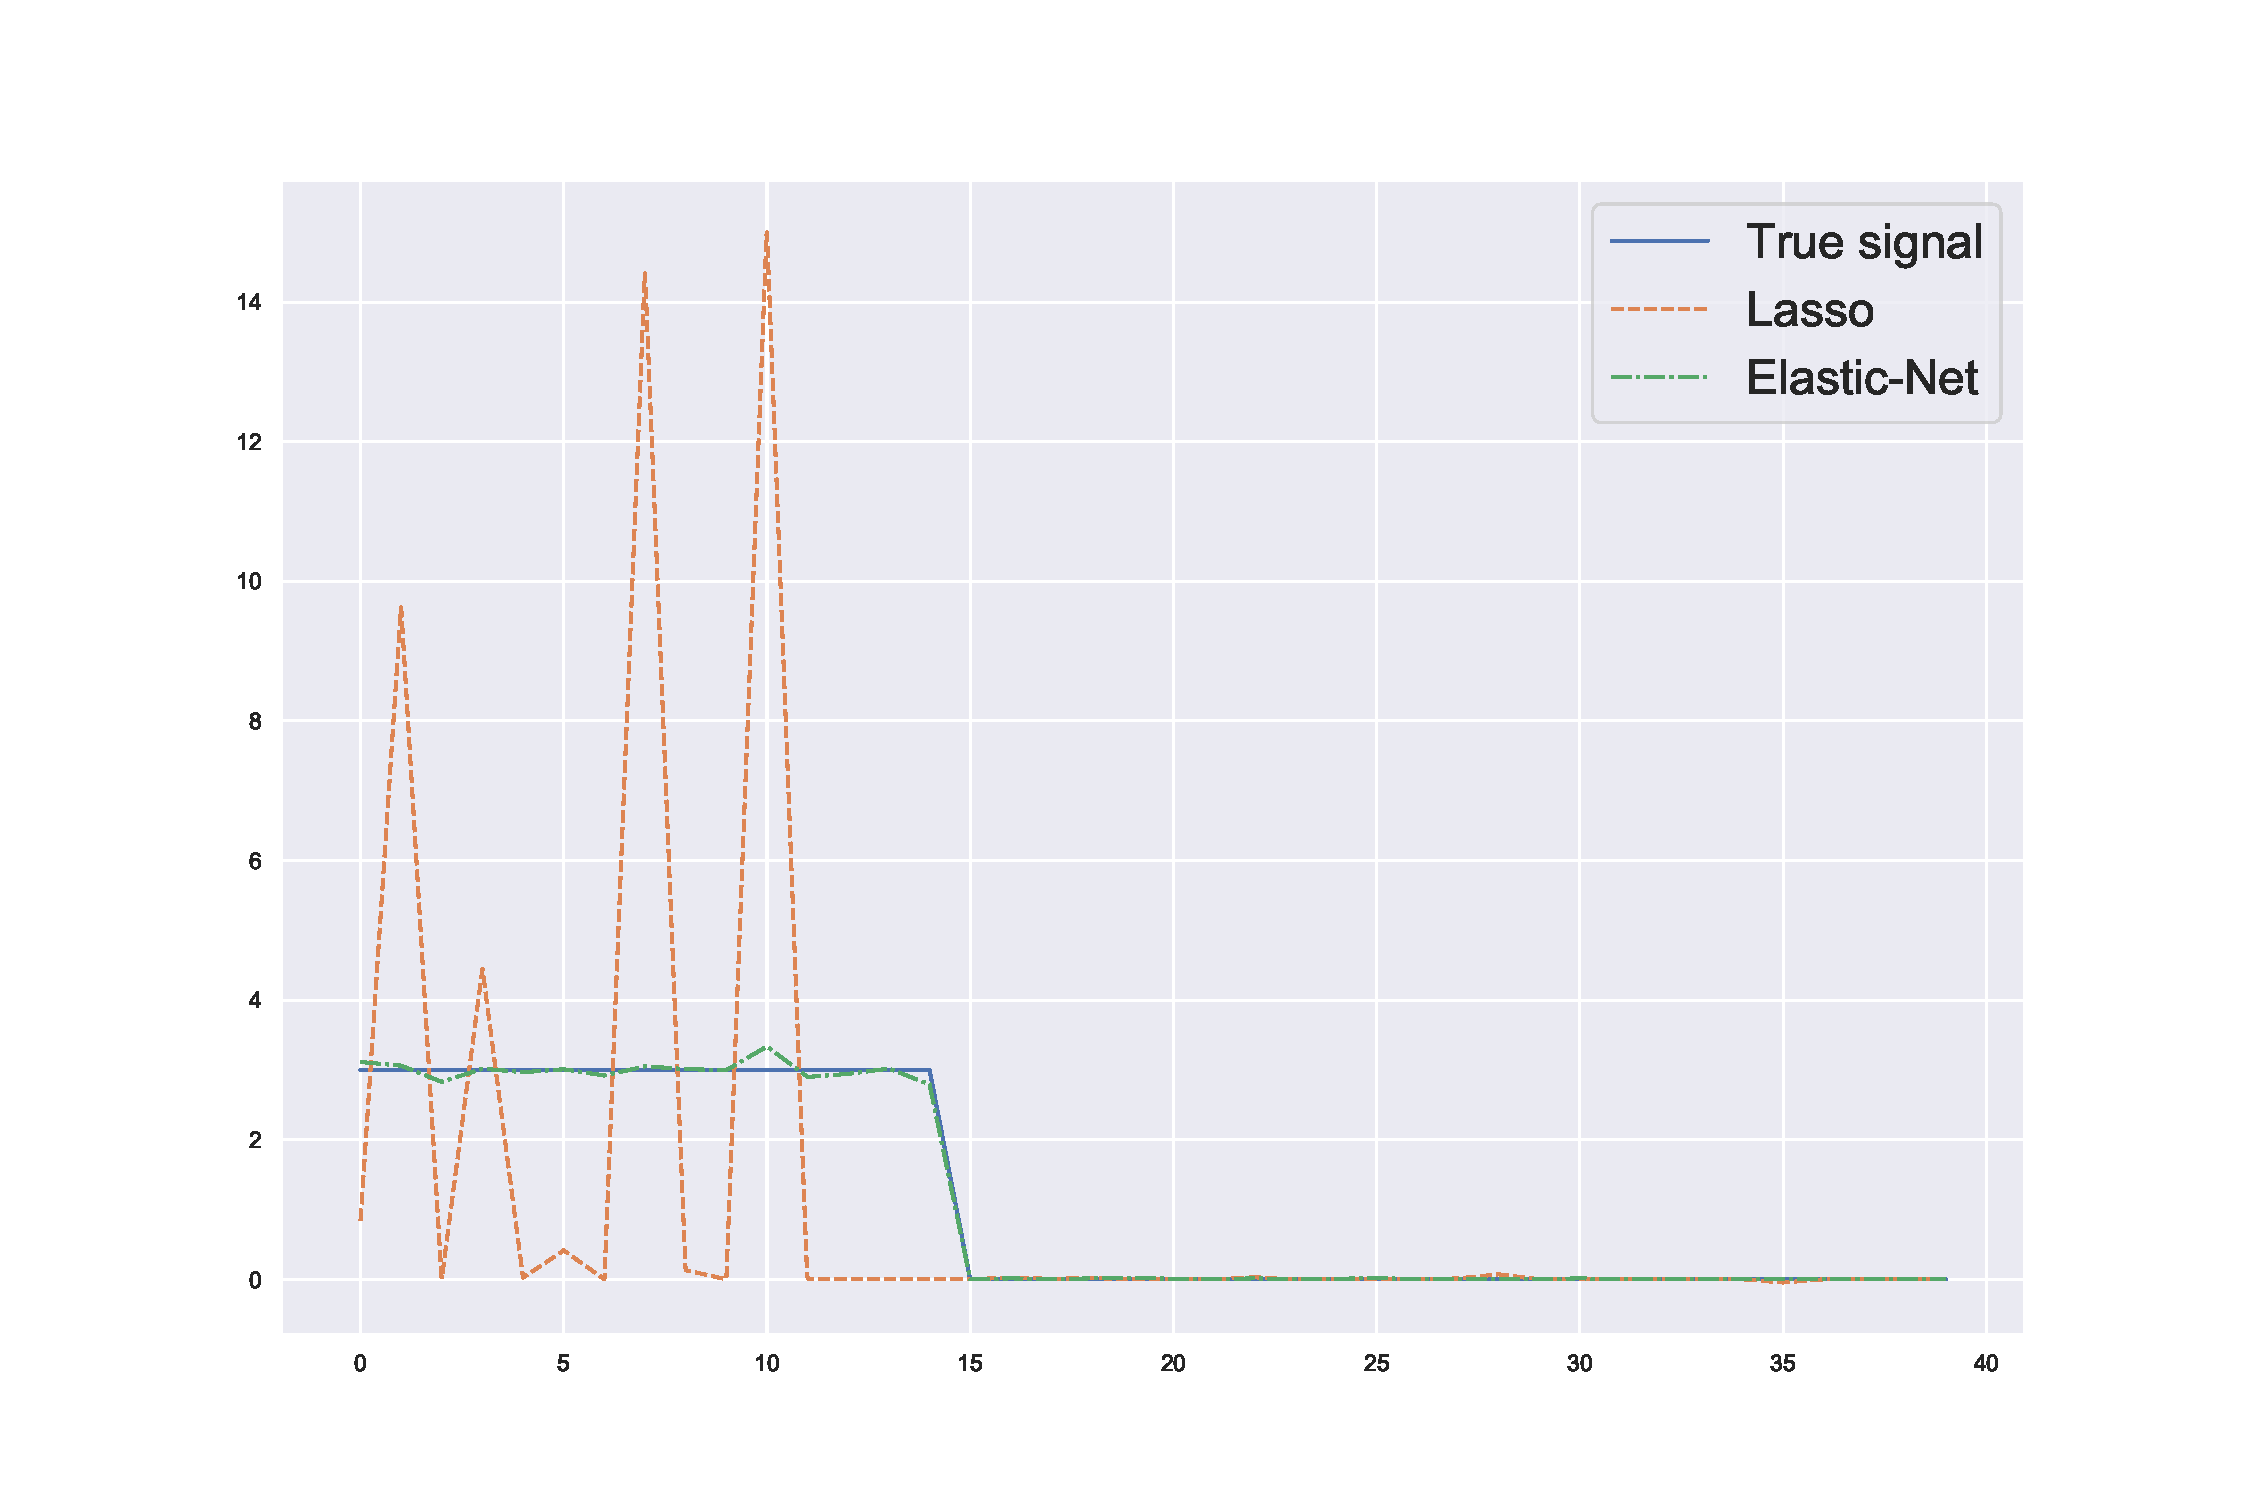
\includegraphics[width=.9\linewidth]{Lasso_enet.pdf}
        \caption{Representation of the grouping effect of the LASSO in a highly correlated situation and how the Elastic net is better is that case.}
        \label{fig:lasso_enet}
    \end{figure}
\end{center}



% the studied penalty
The proposition of \textbf{MAKE CITATION} is to keep the $l_0$ norm for the sparsity penalty and use the $l_2$ norm in the \enet for the grouping effect. The penalty is then:
\[s_k(x)=\begin{cases} \frac{1}{2}\|x\|_2^2, \text{ if } \|x\|_0\leq k\\
\infty, \text{ else}\end{cases} = \frac{1}{2}\|x\|_2^2 + \delta_{C_k}\enspace.\]
However, the first problem is still there. We don't have neither the continuity nor the convexity. That's why instead of considering $s_k$, we will consider it's best convex estimator, the sparse envelope:
\[ \mathcal{S}_k(x) := s_k^{**}(x)\enspace,\]
where, for a function $f$, we define its convex conjugate (also called Fenchel's conjugate) by  
\begin{equation}\label{eq:conjugate}
    f^*(y)=\max_{x\in\RR^n}\{\langle x, y\rangle - g(x)\}\enspace.
\end{equation}
Our goal from now is to compute efficiently the proximal operator of $\lambda \mathcal{S}_k$, for $\lambda >0$ and then compare our results to the \enet ones.


%%%%%%%%%%%%%%%%%%%%%%%%%%%%%%%%%%%%%%%%%%%%%%%%%%%%%%%%%%%%%%%%%%%%
% Sections 2: s** = S (what is this object?)
%%%%%%%%%%%%%%%%%%%%%%%%%%%%%%%%%%%%%%%%%%%%%%%%%%%%%%%%%%%%%%%%%%%%
\section{Compute the convex biregularization}
% Introduce H_k and the problem
First, let's note $\abs{x_{\langle i\rangle}}$ the $i\textsuperscript{th}$ biggest (in absolute value) component of the vector $x$. The best approximation (w.r.t the $l_2$ norm) in $C_k$ for a determined $k\in\NN^*$ of a signal $x\in\RR^n$ is noted $H_k(x)$ and we define its components with 
\[\big(H_k(x)\big)_j = \begin{cases} x_j,\text{ if }x_j \geq \abs{x_{\langle k\rangle}} \\
0, \text{ else }\end{cases} \forall j =1,\dots, n\enspace. \]
Now, we can try to find an expression for $\mathcal{S}_k(x)$.

% Proposition conjugate of s
\begin{proposition}\label{prop:skstar}
Let $y\in\RR^n$ and $k\in\NN^*$, then $s_k^*(y) = \frac{1}{2}\|H_k(y)\|^2_2$.
\end{proposition}

% its proof
\begin{proof}
Using \eqref{eq:conjugate}, we know that for $y\in\RR^n$,
\[
\begin{aligned}
s_k^*(y) & = \max_{x\in\RR^n}\left[\langle x,y\rangle - s_k(x)\right] = \max_{x\in\RR^n}\left[\langle x,y\rangle - \frac{\|x\|_2^2}{2}\right]\\
         & = \max_{x\in\RR^n}\left[-\left(\frac{\|x\|^2_2}{2} - \langle x, y\rangle\right) \right]
         & = \max_{x\in\RR^n}\left[-\frac{\|x-y\|^2_2}{2} + \frac{\|y\|^2_2}{2} \right] \enspace.
\end{aligned}
\]
Besides, $H_k(x)\in\arg\min_{y\in C_k}\|x-y\|_2$ and $\|y\|_2^2$ is independent of $x$, so 
\[s_k^*(y) -\frac{1}{2}\|H_k(y) - y\|^2_2 + \frac{1}{2}\|y\|_2^2\enspace.\]
And $-\|H_k(y) -y\|^2_2 = -\|H_k(y)\|_2^2 - \|y\|^2_2 + 2 \langle H_k(y),y\rangle$. But because $(H_k(y))_j=0$ for the $n-k$ smallest absolute values of $y$, $\langle H_k(y),y\rangle = \|H_k(y)\|_2^2$. Thus, we obtain by plugging-in this value:
\[s_k^*(y) = -\frac{1}{2}\|H_k(y)\|_2^2\enspace.\]
\end{proof}

% Begin the biconjugate expression
To find the biconjugate of $s_k(y)$, we now only have to find the conjugate of $-\frac{1}{2}\|H_k(y)\|^2_2$. Let's introduce the space $D_k=\{u\in\RR^n\,|\,\sum_{i=1}^n u_i \leq k,\  0\leq u_i\leq 1\ \forall i\}$. Then 
\begin{equation}\label{eq:minmax}
\mathcal{S}_k(x) = \max_{y\in\RR^n}\min_{u\in D_k}\left\{\langle x, y\rangle - \frac{1}{2}\sum_{i=1}^n u_iy_i^2\right\}\enspace.
\end{equation}
Thanks to Sion's $minimax$ theorem \cite{10.2307/30037472} thanks to the convexity and concavity, we can inverse the $\min$ and $\max$ we can switch the two operators and get an expression of $\mathcal{S}_k(x)$.

% theorem with the linear over quadratic formula
\begin{proposition} With the same notations we have 
\begin{equation}\mathcal{S}_k(x) = \frac{1}{2}\min_{u\in D_k} \sum_{i=1}^n \phi(x_i, u_i)\text{, where }
\phi(x,u)=\begin{cases}\frac{x^2}{u},&\ \text{if }u>0\\ 0&\ \text{if }u=x=0\\ \infty &\text{else} \end{cases}\enspace.\end{equation}
\end{proposition}
\begin{proof}
We only have to consider the inner part of \eqref{eq:minmax}. Let $i_0\in\{1,\dots,n\}$ an index. We want to find the value at the optimum so we get
\[ \frac{\partial}{\partial y_{i_0}} \sum_{i=1}^n x_iy_i -\frac{1}{2}\sum_{i=1}^n u_iy_i^2 = x_{i_0} - \frac{1}{2}2u_{i_0}y_{i_0}\enspace.\]
At the optimum, equalizing to $0$, if $u_{i_0}>0$ we indeed get $\hat y_{i_0} = \frac{x_{i_0}}{u_{i_0}}$ and the other values are trivial in the other cases. Plugging-in the obtained value, we finally get the result for $u_i>0$ (the other cases are direct):
\[\max_{y\in\RR^n}\left\{x'y - \frac{1}{2}\sum_{i=1}^nu_iy_i^2\right\} = \sum_{i=1}^nx_i \frac{x_i}{u_i} - \frac{1}{2}\sum_{i=1}^n u_i \frac{x_i^2}{u_i} = \frac{1}{2}\sum_{i=1}^n \frac{x_i^2}{u_i}\enspace.\]
\end{proof}

% expression for S_k(x)
From there, it can be proved \cite{beck}, that if $\|x\|_0\leq k$ then $\mathcal{S}_k(x)=\|x\|_2^2 /2$. Otherwise, the expression depends on the root of a function defined as the sum of linear monotonous piecewise functions with a single breakpoint:
\[g_x(\eta)=\sum_{i=1}^n \min\{\abs{x_i}\eta,1\} - k,\ \eta\geq 0\enspace.\]
The general expression of $\mathcal{S}_k(x)$ is:
\begin{equation}
    S_k(x)=\frac{1}{2}\sum_{i=1}^{N_x} x_{\langle i \rangle}^2 + \frac{1}{2(k- N_x)}\left(\sum_{i=N_x+1}^n\abs{x_{\langle i\rangle}}^2\right)^2\enspace,
\end{equation}
where $N_x=\arg\max_{i=1,\dots,n}\left\{\abs{x_{\langle i\rangle}}\geq\tilde\eta ^{-1}\right\}$, with $\tilde \eta$ the root of $g_x$.

%%%%%%%%%%%%%%%%%%%%%%%%%%%%%%%%%%%%%%%%%%%%%%%%%%%%%%%%%%%%%%%%%%%%
% Sections 3: prox_lambdaSk (comparisons with Enet)
%%%%%%%%%%%%%%%%%%%%%%%%%%%%%%%%%%%%%%%%%%%%%%%%%%%%%%%%%%%%%%%%%%%%
\section{Proximal operator computation and numerical results}
\subsection{Compute the proximal operator}

\subsection{Numerical application}
Let's finally compare our regularized problem with the \enet
regularization in an highly correlated situation (the same represented in Figure \ref{fig:lasso_enet}).
We simulate a signal with only $3$'s for the first fifteen components and zeros for the rest. The observed signal is 
\[ b = Ax + \varepsilon\enspace,\]
where $\varepsilon\sim\mathcal{N}(0,\sigma^2)$ is a Gaussian noise.

% keep describing A

The sparse-envelope problem is written as:
\[\min_{x\in \RR^n} \|Ax-b\|^2_2 + \lambda\mathcal{S}_k(x)\enspace,\]
where $\lambda$ must be chosen through a train/test procedure and we take $k=15$ because we know its real value here otherwise we would have to search it as well.

\begin{center}
    \begin{figure}
        \centering
        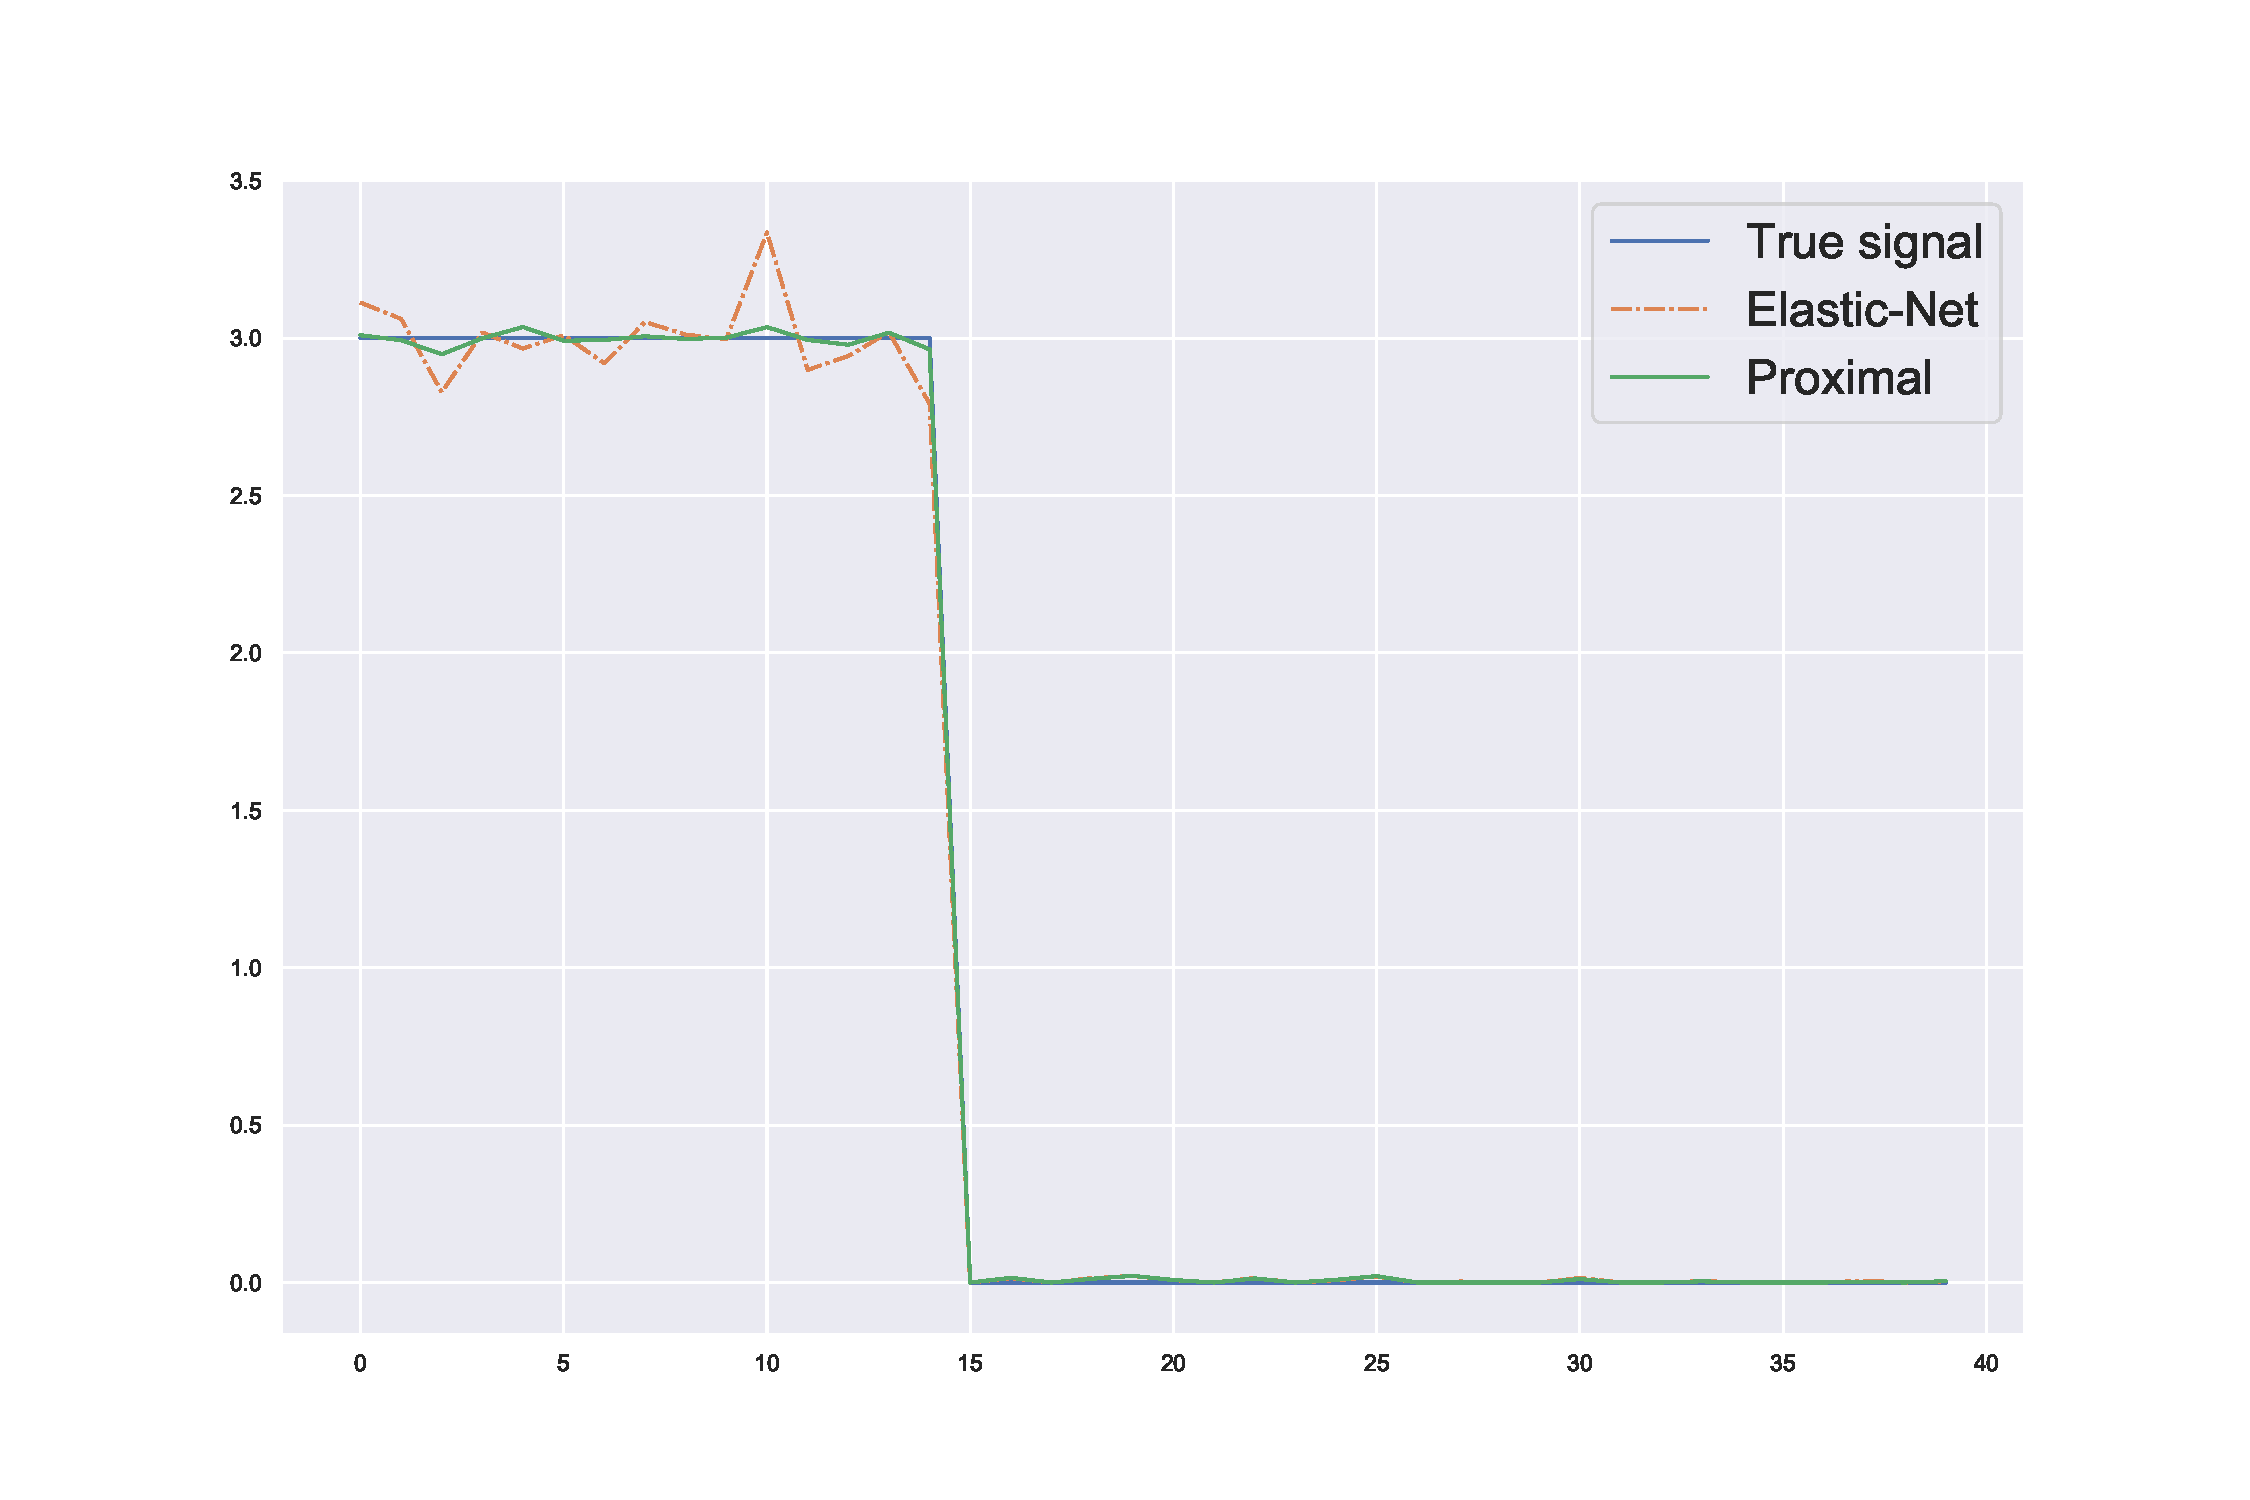
\includegraphics[width=.9\linewidth]{enet_proxi.pdf}
        \caption{Comparison of the Elastic-net and sparse regularization in a highly correlated situation with $n=50$ and $\sigma=0.1$.}
        \label{fig:enet_sp}
    \end{figure}
\end{center}

As the Figure \ref{fig:enet_sp} shows, the proximal envelope is even closer to the original signal than the \enet in this case.
We can now compare if this is also the case for some increasing values of $n$ and quantify the gain of using this method instead of the \enet currently used.

%%%%%%%%%%%%%%%%%%%%%%%%%%%%%%%%%%%%%%%%%%%%%%%%%%%%%%%%%%%%%%%%%%%%
% Conclusion
%%%%%%%%%%%%%%%%%%%%%%%%%%%%%%%%%%%%%%%%%%%%%%%%%%%%%%%%%%%%%%%%%%%%

\section*{Conclusion}

In conclusion, the biregularization method................


%%%%%%%%%%%%%%%%%%%%%%%%%%%%%%%%%%%%%%%%%%%%%%%%%%%%%%%%%%%%%%%%%%%%%%%%%%%%%
%%%%%%%%%%%%%%%%%%%%%%%%%%    Bibliography   %%%%%%%%%%%%%%%%%%%%%%%%%%%%%%%%
%%%%%%%%%%%%%%%%%%%%%%%%%%%%%%%%%%%%%%%%%%%%%%%%%%%%%%%%%%%%%%%%%%%%%%%%%%%%%

\section{Bibliography}
\nocite{*}
\printbibliography


\end{document}
